\section{Proposed Model}

\begin{figure}[h]
    \centering
    \includegraphics[width=0.7\textwidth]{graphics/architecture.png}
    \caption{The modular architecture of the proposed \textbf{ClimateSAM} model. The architecture features trainable components—the Input Adapter, Encoder Adapter, and Geometric Prompt Generator—while the core SAM Image Encoder is kept frozen. The Encoder Adapter Architecture architecture incorporates a decoupled design, has separate HQ-prompt tokens, prompt adapters and dedicated MLPs for each task (TC and AR), while the rest of components are shared.}
    \label{fig:climatesam_arch}
\end{figure}

The proposed \textbf{ClimateSAM architecture}, illustrated in Figure \ref{fig:climatesam_arch}, is a modular framework designed for climate pattern segmentation. It begins with an \textbf{Input Adapter} that performs dimensionality reduction, compressing the 16 input climate variables into a 3-channel tensor, analogous to an RGB image. This tensor is then fed into a pre-trained SAM \textbf{Image Encoder}, which remains frozen to leverage its powerful, pre-existing feature extraction capabilities.

To adapt the model to the climate domain, a parameter-efficient \textbf{Encoder Adapter} injects a set of learnable prompt tokens into each transformer layer \cite{xiao2024cat}. To effectively handle the dual-task learning of distinct phenomena (AR vs TC), this adapter is enhanced with two separate, high-quality prompt tokens \cite{ke2023segment}. Each token is managed by a dedicated prompt bridge (a 2-layer MLP), decoupling the learning pathways to mitigate task interference and enable specialized feature adaptation.

An automated \textbf{Geometric Prompt Generator} utilizes intermediate outputs from the vision transformer layers, applying multi-scale fusion and thresholding to dynamically generate point prompts \cite{chen2024sam}. Finally, the \textbf{Mask Decoder} integrates these point prompts, the image features from the encoder, and the task-specific tokens. These tokens are processed through a 3-layer MLP to generate dynamic weights, which are then used to produce the final segmentation masks.

The following sections will explain the choice of the architecture.

\section{Tuning Image Encoder}
We employ prompt tuning, a Parameter-Efficient Tuning (PET) technique, to adapt the heavyweight image encoder of the SAM architecture while keeping its original weights frozen. Drawing from the CAT-SAM-T architecture \cite{xiao2024cat}, we use a decoder-conditioned joint tuning strategy tailored for SAM. This method introduces a set of learnable tokens, alongside the input patch embeddings. CAT-SAM-T introduces a CAT-Token that is mapped to prompt tokens by passing through a prompt bridge (a two-layer MLP), which are later injected into each transformer layer of the image encoder. These, along with the CAT-Token and the weights of the MLP in the mask decoder, are the parameters updated during the adaptation process.

The proposed method operates by keeping the entire pre-trained decoder of the SAM frozen. The learnable CAT-Token is concatenated with SAM's original prompt and output tokens (including mask and IoU tokens). This combined set of tokens serves as the input to the frozen SAM decoder layers. A key aspect of this method is that the updated CAT-Token is independently processed to generate dynamic weights for a new three-layer Multi-Layer Perceptron (MLP). This MLP is subsequently used to generate the refined target masks.

\section{Individual Detection vs Dual Detection}
\begin{figure}[h!]
    \centering
    
    % --- Graphic (a) ---
    % minipage is set to \textwidth, so the two graphics stack vertically
    \begin{minipage}{\textwidth}
        \centering
        % Image (a)
        \includegraphics[width=0.8\textwidth]{graphics/Cat-sam.png}
        
        \vspace{0.2cm} % Small vertical space below the image

        % Manual "Subcaption" (a)
        \centering
        \parbox{0.8\textwidth}{\centering
            \textbf{(a)} Cat-SAM performance on a climate dataset for single detection (TC or AR), utilizing geometric prompts generated from true masks.
        }
        \label{fig:catsam_single}
    \end{minipage}

    \vspace{0.5cm} % Adds vertical space between the two graphics

    % --- Graphic (b) ---
    \begin{minipage}{\textwidth}
        \centering
        % Image (b)
        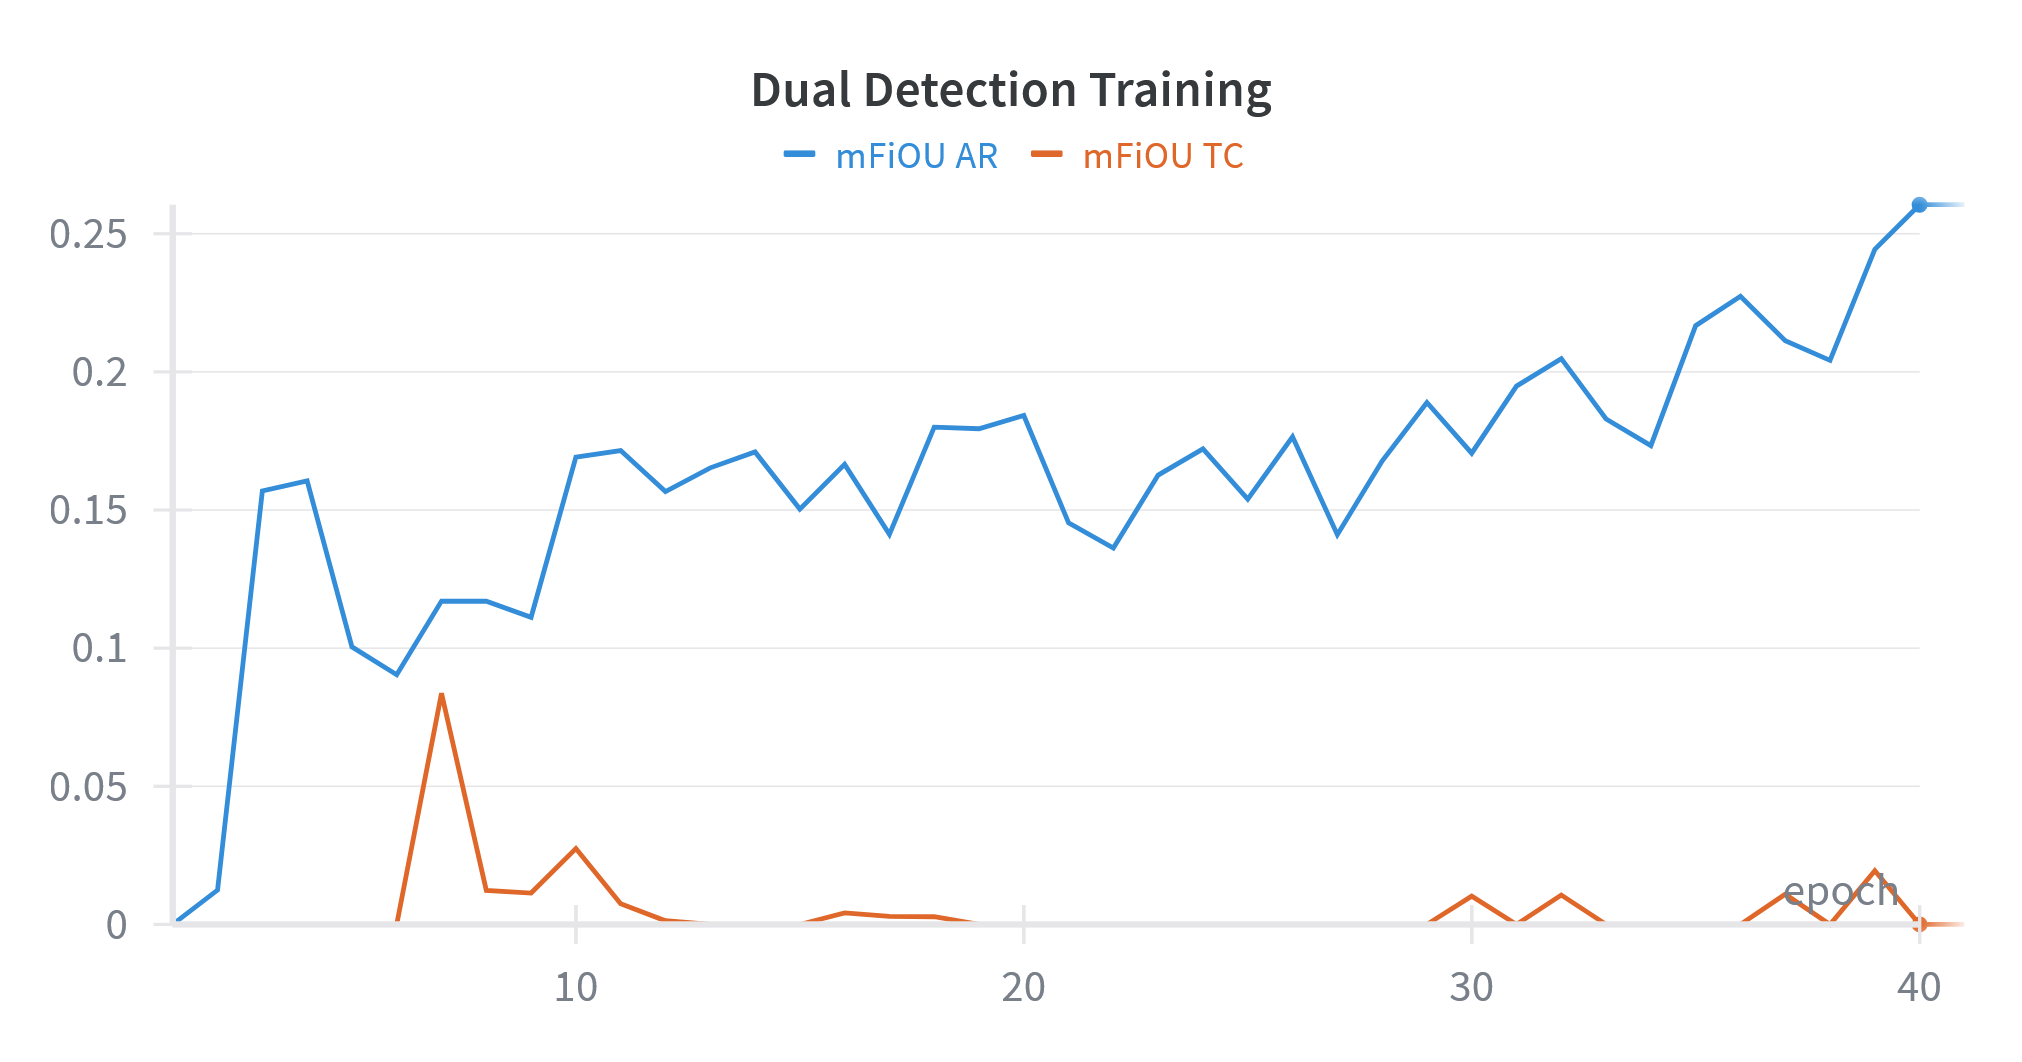
\includegraphics[width=0.8\textwidth]{graphics/dual_long.png}
        
        \vspace{0.2cm} % Small vertical space below the image

        % Manual "Subcaption" (b)
        \centering
        \parbox{0.8\textwidth}{\centering
            \textbf{(b)} Model performance in dual detection using a single shared Encoder Adapter architecture. The model exhibited difficulty in simultaneously learning both Tropical Cyclone (TC) and Atmospheric River (AR) patterns.
        }
        \label{fig:dual_single_adapter}
    \end{minipage}

    % Combined Main Caption
    \caption{Comparison of model performance across single-task and dual-task learning scenarios. (a) shows the high performance achievable when focusing on one climate pattern (Cat-SAM), and (b) illustrates the performance degradation when forcing a single-adapter architecture to learn both TC and AR simultaneously.}
    \label{fig:performance_comparison}
\end{figure}

To empirically validate the performance of the CAT-SAM architecture, the model was evaluated using ground truth geometric prompts derived from annotated labels. The architecture was trained independently on datasets for AR and TC Due to the significant class imbalance, where the spatial extent of TC and AR regions is considerably smaller than the background, the mean Foreground Intersection over Union (mFIoU) was selected as the primary evaluation metric to mitigate potential bias. 

The empirical results demonstrate that CAT-SAM achieves superior performance compared to established baseline models. Specifically, the model attained an mFIoU of 70\% with a comparatively reduced training duration, contingent upon the provision of accurate geometric prompts and a distinct feature training regimen.

To investigate the CAT-SAM model's capacity for dual detection of both AR and TC, we trained the architecture using a multi-class configuration.  This preliminary experiment revealed a significant limitation: the model failed to concurrently improve detection metrics for both phenomena. This outcome suggests the model struggled with the joint feature learning necessary to distinguish between and accurately predict both AR and TC regions simultaneously.

Modified Approach:
To address the issue of learning two different tasks being affected when sharing the same encoder adapter, the modified approach uses two distinct HQ prompt tokens. Each of these tokens has its own prompt bridge (adapters) within the image encoder, and there are two separate 2-layer MLPs, one for each token. This is illustrated in Figure \ref{fig:climatesam_arch} This setup ensures that each task can be learned effectively.

\section{Loss Function}

\begin{table}[h]
    \centering
    \caption{Summary of AR and TC Image and Object Metrics}
    \label{tab:summary_stats}
    % Use p{width} for columns where you need wrapping text.
    \begin{tabular}{llccc}
        \toprule
        \textbf{Type} & \textbf{Statistic} & \thead{\textbf{\#Masks} \\ \textbf{per Image}} & \thead{\textbf{Background/} \\ \textbf{Object Pixel Ratio} \\ \textbf{Per mask}}  & \thead{\textbf{Background/} \\ \textbf{Object Pixel Ratio} \\ \textbf{Per Image} } \\
        \midrule
        \multirow{2}{*}{\textbf{AR}}
            & Mean & 7.43 & 351.36 & 2,242 \\
            & Median & 7.00 & 142.23 & 17 \\
        \midrule
        \multirow{2}{*}{\textbf{TC}}
            & Mean & 2.56 & 880.72 & 149,220 \\
            & Median & 2.00 & 685.37 & 257 \\
        \bottomrule
    \end{tabular}
\end{table}

Table \ref{tab:summary_stats} clearly shows the significant class imbalance in the data. To tackle this, we employ a composite loss function that combines a weighted Binary Cross-Entropy (BCE) loss and a Dice loss. This approach effectively mitigates two primary challenges:
\begin{enumerate}
    \item \textbf{Mask Frequency Discrepancy:} The dataset exhibits a notable difference in the number of masks per data point, with TCs averaging 3.6 masks compared to ARs averaging 0.8.
    \item \textbf{Extreme Foreground-to-Background Pixel Ratio:} The prevalence of background pixels is exceptionally high, with median ratios of 16.98 for ARs and 257.24 for TCs.
\end{enumerate}

Furthermore, empirical observations indicate a tendency for the model to output all-zero masks (predicting only background) due to the vastness of the background. To counteract this, the loss function is specifically formulated to penalize false negatives more heavily than false positives. This is achieved through the weighting mechanisms within both the BCE and Dice loss components, ensuring that the model is strongly incentivized to identify and segment foreground objects, even in the presence of overwhelming background information.

The combined loss is structured as follows:
\begin{align*}
    \text{Loss}_{\text{total}} &= \text{Loss}_{\text{TC}} + \text{Loss}_{\text{AR}} \\
    \text{Loss}_{\text{TC}} &= \text{Loss}_{\text{Dice\_TC}} + \text{Loss}_{\text{BCE\_TC}} \\
    \text{Loss}_{\text{AR}} &= \text{Loss}_{\text{Dice\_AR}} + \text{Loss}_{\text{BCE\_AR}}
\end{align*}


\subsection{Training Pipeline}

\begin{table}[h!]
    \centering
    \caption{Parameter Information for Phase 1 of the Training Scheme.}
    \label{tab:phase1_params} % You should give your table a unique label
    \begin{tabular}{l | l | r}
        \hline
        \textbf{Component} & \textbf{Trainable} & \textbf{Trainable Parameters} \\
        \hline
        \texttt{ORI\_SAM} & False & 0 / 89,677,132 (0.00\%) \\
        \texttt{INPUT\_ADAPT} & False & 0 / 51 (0.00\%) \\
        \texttt{MASK\_DECODER} & True & 1,211,168 / 5,269,508 (22.98\%) \\
        \texttt{IMAGE\_ENCODER} & True & 1,593,344 / 91,264,256 (1.75\%) \\
        \texttt{PROMPT\_ENCODER} & False & 0 / 6,220 (0.00\%) \\
        \hline
    \end{tabular}
\end{table}

The phased training approach is implemented to address computational constraints and facilitate the learning of robust feature representations from input data. This methodology also mitigates parameter forgetting, as a prompt generator's efficacy is contingent upon the model's ability to effectively represent image features.

To enable the tuning of the image adapter and mask decoder in the absence of an automated prompt generator and input adapter, two strategies are employed:

\begin{enumerate}
    \item \textbf{Input Data Normalization:} Following the methodology proposed by Radke \cite{radke2024explaining}, the three most critical parameters for detection—TMQ, U80, and V80—are utilized. These variables are normalized and presented to the model as a three-channel RGB input. This normalization ensures a consistent image distribution for tuning the encoder adapter.
    
    \item \textbf{Geometric Prompt Generation:} For the geometric prompt generators, point and box prompts are derived from the ground truth labels of the objects. The extraction pipeline is detailed in Figure 1. Upon invoking a dataset item, a uniform random decision is made to determine whether point prompts or box prompts will be provided. Point prompts are generated by randomly selecting a pixel coordinate within the object, with a 10\% preference given to centroid points.
\end{enumerate}

The training regimen is conducted on a per-object basis, while validation is performed per image. Given that SAM is designed as an instance segmentation model, per-object training offers a more straightforward supervision mechanism, particularly when prompts are object-specific. Each object is associated with a clear ground truth mask and a defined prompt (either a point or a box). While validation per image assesses if the model can segment all objects accurately in a full image with multiple prompts, evaluated by foreground mIoU. So is the proposed training pipeline:
\begin{itemize}
    \item \textbf{Phase 1:} The Image Adapter and Mask Decoder are trained, while all other components remain frozen. The Table \ref{tab:phase1_params} shows the information of trainable parameters in phase 1.
    \item \textbf{Phase 2:} The Input Adapter is trained, with all other components frozen.
    \item \textbf{Phase 3:} The Prompt Generator is trained, with the Image Adapter and Mask Decoder frozen.
\end{itemize}

\section{Geometric Prompt Generator}


\begin{figure}[h]
    \centering
    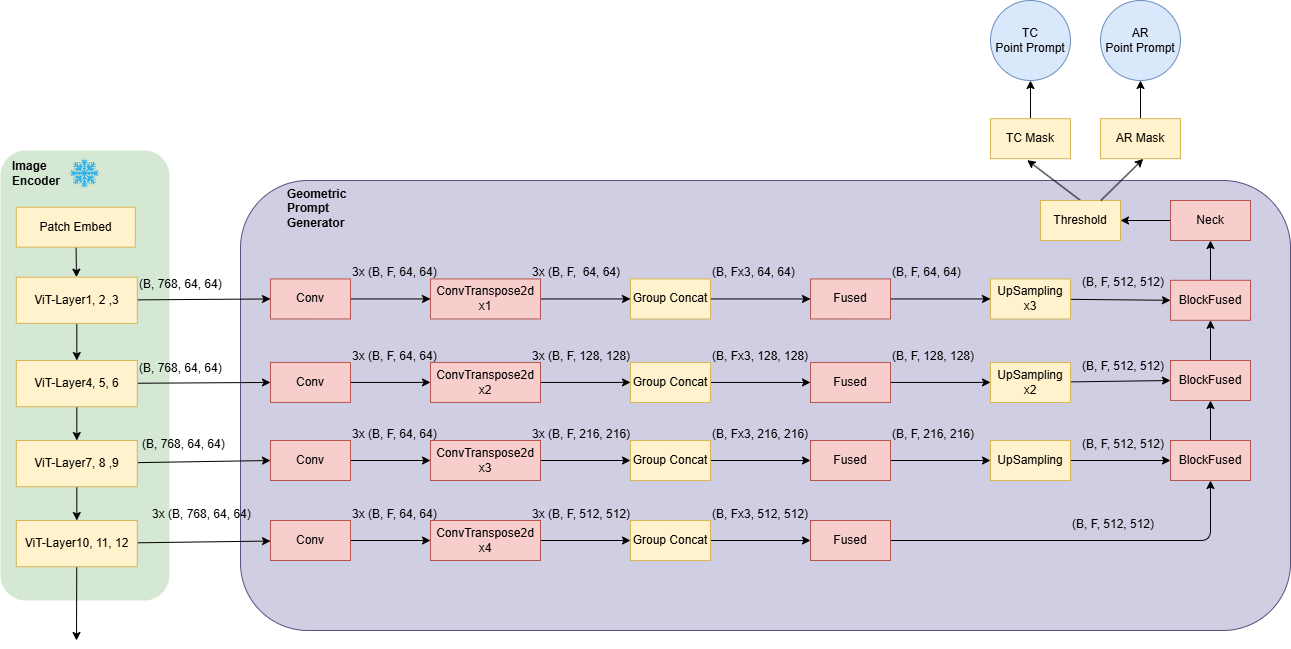
\includegraphics[width=0.9\textwidth]{graphics/prompt.png}
    \caption{Prompt Generator Architecture with mask size of 518}
    \label{fig:prompt_gen}
\end{figure}



The automatic geometric prompt generator is implemented following the completion of Phase 2 training. This sequential approach ensures that the image and mask encoders are sufficiently trained to produce robust feature representations, which are essential for the effective operation of the prompt generator.

The proposed architecture is a multi-scale self-prompt generation mechanism, adapted from the Un-SAM mode \cite{xie2025self, xie2024masksam}. It leverages the intermediate feature maps, from the vision transformer layers. These feature maps are fed into multiple convolutional heads with different strides to produce embeddings at various scales. Subsequently, a Feature Pyramid Network (FPN) integrates these multi-level features via a top-down pathway. Finally, the output from the FPN is passed through a thresholding mechanism to select the final point prompts for segmentation. Figure \ref{fig:prompt_gen} illustrates the architecture.


\begin{enumerate}

    \item \textbf{Channel Reduction and Upsampling:} Each of the three input features per block is first passed through a $1 \times 1$ convolution to reduce the channel dimension from $\text{in\_channels}$ to $\text{fused\_channels}$. These features are then spatially upsampled using a varying number of \textbf{transposed convolutions} ($\texttt{ConvTranspose2d}$), where the degree of upsampling increases with each block index ($n+1$ layers for Block $n$).

    \item \textbf{Group Fusion and Iterative Aggregation:} The three upsampled features are concatenated along the channel dimension ($3 \times \text{fused\_channels}$) and fused via a $1 \times 1$ convolution, followed by a $3 \times 3$ convolution which applies a spatial downsampling (stride 2). For subsequent blocks, the newly fused feature is \textbf{concatenated} with the upsampled output of the previous block, creating an iterative information flow. This combined feature is then upsampled by a factor of 2 using bilinear upsampling ($\texttt{Upsample}$) for the next block.

    \item \textbf{Output Generation:} The final aggregated feature map is passed through a neck layer ($1 \times 1$ Conv) for final channel reduction. This feature then feeds two identical convolutional heads ($\texttt{mask1\_conv}$ and $\texttt{mask2\_conv}$), each using two strided convolutions (with grouped channels in the first layer) to produce the final, single-channel $\texttt{tc\_mask}$ and $\texttt{ar\_mask}$ outputs.

\end{enumerate}

\vspace{-1mm}

\noindent The overall process efficiently aggregates information from multiple encoder stages while iteratively increasing the spatial resolution towards the final mask outputs.


\section{Timeline}
\subsection*{Phase 1: Domain Adaptation Problem Solving (Completed) $\mathbf{\rightarrow}$ Target: 2025-10-15}
Establish the foundational approach and resolve the core domain adaptation challenge.
\begin{itemize}
    \item Literature research.
    \item Solve the domain adaptation problem with the proposed architectural design (Decoupled HQ-Token).
\end{itemize}

\subsection*{Phase 2: Prompt-Free Baseline Generation $\mathbf{\rightarrow}$ 2025-11-15}
Develop a fully prompt-free ClimateSAM as a baseline, without necessarily outperforming results, using an auxiliary network.
\begin{itemize}
    \item Use CGNet for generating auxiliary masks, processing them to give geometric prompts.
    \item Train the input adapter.
\end{itemize}

\subsection*{Phase 3: Prompt Generator Finalization $\mathbf{\rightarrow}$ 2025-12-31}
Integrate intermediate embedding into the prompt generator.
\begin{itemize}
    \item Adapt the current architecture to leverage image encoding to generate a Confidence Map (MAP), which subsequently informs an Adaptive Sampling and Filtering Component. This component will be inspired by the principles of AoP-SAM and SAM-SP \cite{chen2025aop, zhou2024sam}.
    \item Modify the current architecture to incorporate immediate embeddings derived from Vision Transformer (ViT) layers, as to create a multi-scale prompt generator, inspired by Un-SAM and MaskSAM \cite{xie2025self, xie2024masksam}.
\end{itemize}

\subsection*{Phase 4: Optimization and Validation $\mathbf{\rightarrow}$ 2026-01-31}
Refine the system's efficiency and other experiments.
\begin{itemize}
    \item Rescale the proposed architecture to significantly reduce computational resource consumption.
    \item Experimentally evaluate the impact of various augmentations and different hyperparameters on model performance.
    \item Experiment the performance of LoRA vs current prompt token approach.
    \item Systematically perform hyperparameter tuning to maximize model efficacy.
\end{itemize}


\subsection*{Phase 5: Documentation and Submission $\mathbf{\rightarrow}$ 2026-02-28}
Finalize the academic documentation and complete the thesis submission process.
\begin{itemize}
    \item Thesis Writing: Compose and refine the final thesis document.
    \item Submission: Complete the formal submission of the thesis.
\end{itemize}


\chapter{Preliminary Result}
In preliminary training, the proposed model, after completing phases 1 and 2 (with given perfect geometric prompts from true masks), significantly surpassed the baseline performance. This training incorporated three augmentation techniques: horizontal flipping, vertical flipping, and horizontal cyclic shifting, the prompt types in training are chosen randomly point, bounding box, or mask. The prompt types for validation is chosen randomly between point and bounding box.

\begin{table}[h!]
    \centering
    \caption{Segmentation Performance Metrics for Climate Events}
    \label{tab:climate_sam_metrics}
    \begin{tabular}{lccc}
        \toprule
        Category & mIoU & mIoU (w/ Background) & Mean Accuracy \\
        \midrule
        Atmospheric Rivers (ARs) & $0.5084$ & $0.7351$ & $0.8289$ \\
        Tropical Cyclones (TCs) & $0.6095$ & $0.8035$ & $0.8435$ \\
        \bottomrule
    \end{tabular}
\end{table}

\begin{figure}[h!]
    \centering
    
    % First Row (a) and (b)
    \begin{minipage}[t]{0.49\textwidth} % Adjust width to 49% for spacing
        \centering
        % Image (a)
        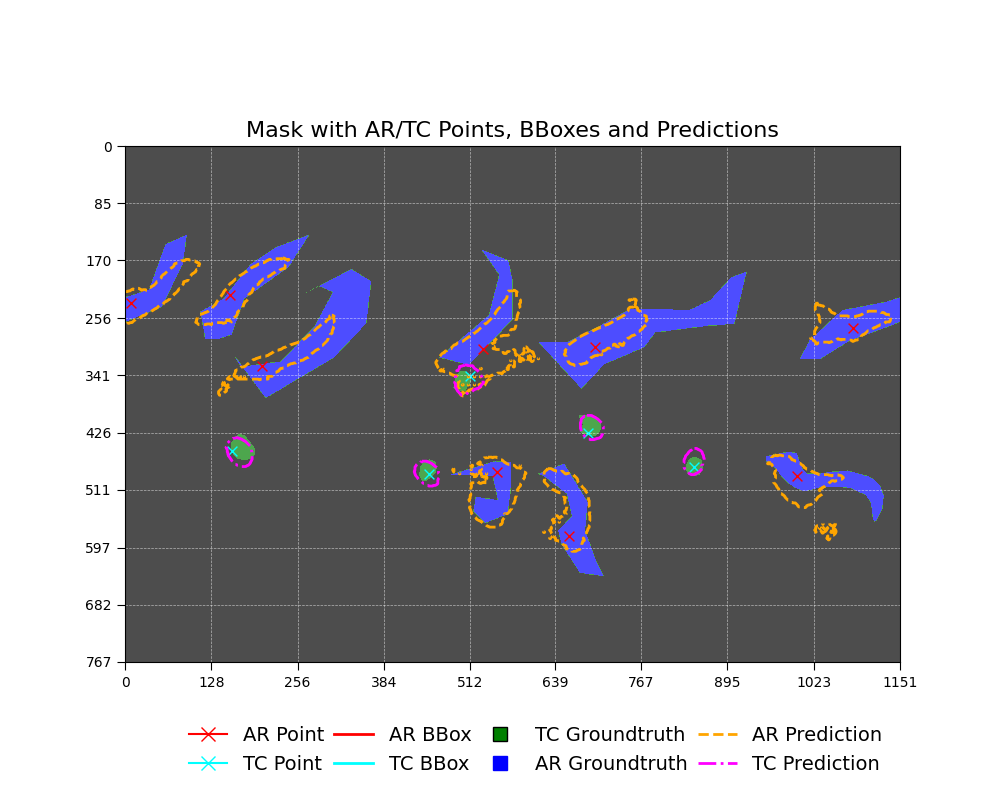
\includegraphics[width=\textwidth]{graphics/valid_1.png} % Image uses full minipage width
        
        \vspace{0.2cm}

        % Subcaption (a)
        \parbox{\textwidth}{\centering
            \textbf{(a)} 
        }
        \label{fig:valid_1}
    \end{minipage}
    \hfill % Horizontal space between minipages
    \begin{minipage}[t]{0.49\textwidth}
        \centering
        % Image (b)
        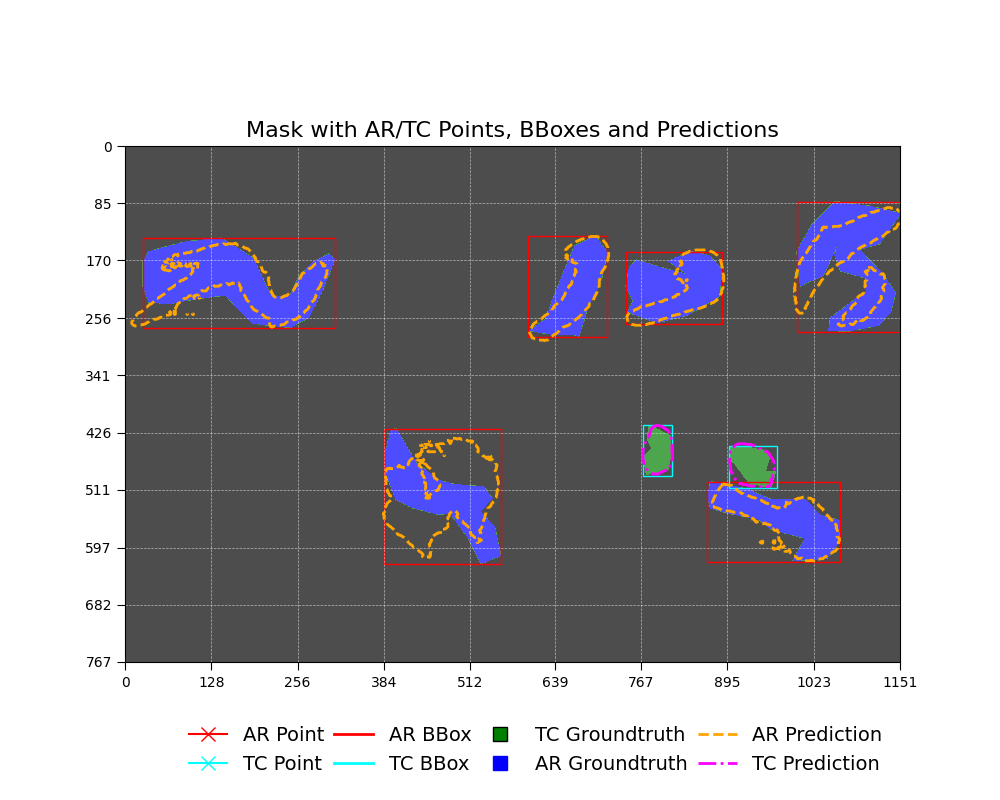
\includegraphics[width=\textwidth]{graphics/valid_2.png}
        
        \vspace{0.2cm}

        % Subcaption (b)
        \parbox{\textwidth}{\centering
            \textbf{(b)} 
        }
        \label{fig:valid_2}
    \end{minipage}

    \vspace{0.5cm} % Vertical space between rows

    % Second Row (c) and (d)
    \begin{minipage}[t]{0.49\textwidth}
        \centering
        % Image (c)
        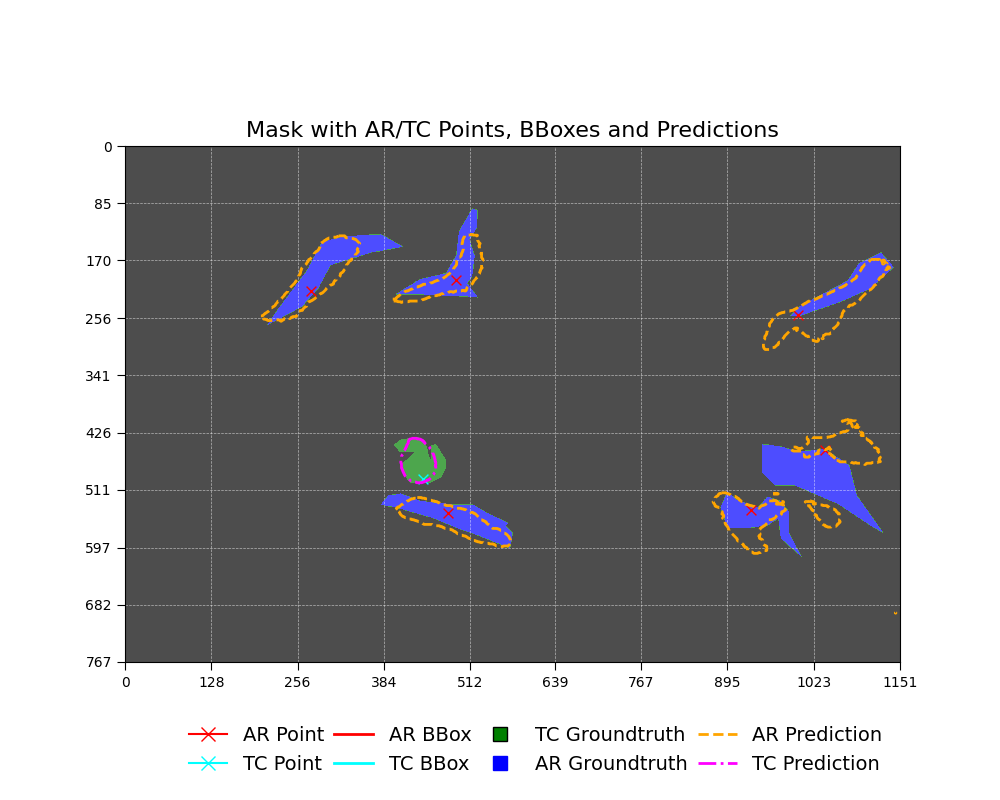
\includegraphics[width=\textwidth]{graphics/valid_3.png}
        
        \vspace{0.2cm}

        % Subcaption (c)
        \parbox{\textwidth}{\centering
            \textbf{(c)} 
        }
        \label{fig:valid_3}
    \end{minipage}
    \hfill
    \begin{minipage}[t]{0.49\textwidth}
        \centering
        % Image (d)
        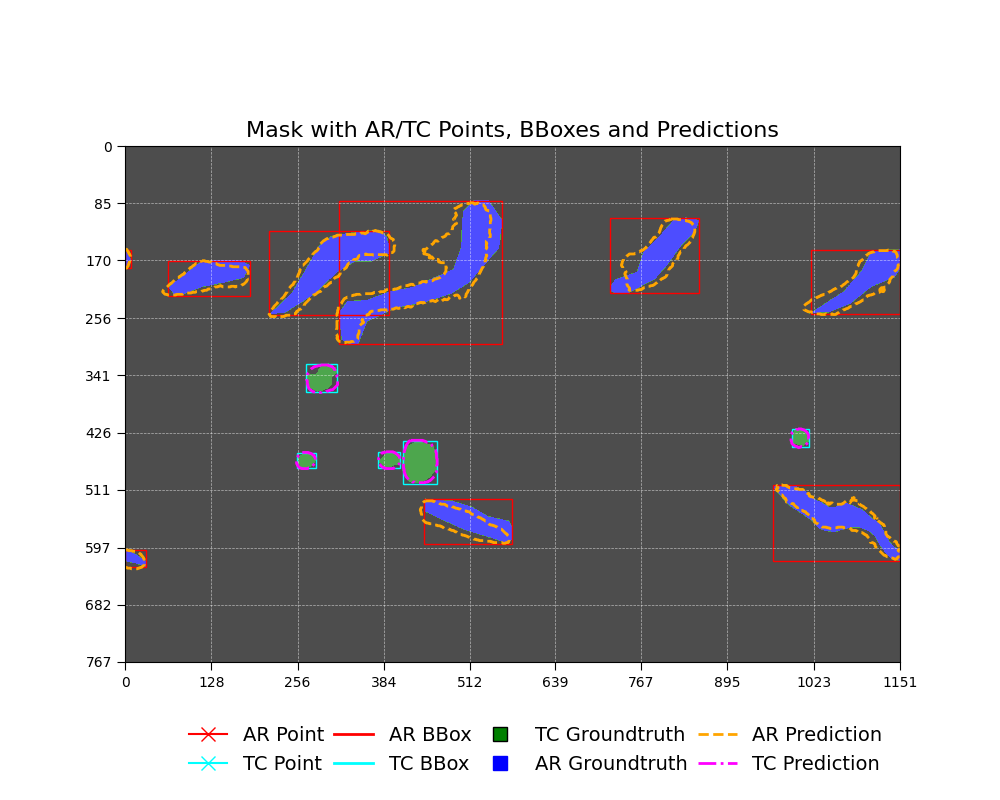
\includegraphics[width=\textwidth]{graphics/valid_4.png}
        
        \vspace{0.2cm}

        % Subcaption (d)
        \parbox{\textwidth}{\centering
            \textbf{(d)} 
        }
        \label{fig:valid_4}
    \end{minipage}

    % Combined Main Caption
    \caption{Valid image at end of training phase for 4 valid examples.}
    \label{fig:valid_examples}
\end{figure}